% Method diagram: residual context-answer mapping (MATS 2026 poster)
% Compile: lualatex -interaction=nonstopmode method_diagram.tex  (pdflatex also works)
\documentclass[tikz,border=6pt]{standalone}
\usetikzlibrary{positioning,calc,decorations.pathreplacing,arrows.meta}
\usepackage{amsmath}
\renewcommand{\familydefault}{\sfdefault}

% ---- palette -------------------------------------------------------------
\definecolor{ctxblue}{HTML}{0072B2}   % v_C
\definecolor{ansgreen}{HTML}{009E73}  % v_A
\definecolor{predorange}{HTML}{E69F00}% \hat v_A
\definecolor{brand}{HTML}{800020}     % MATS maroon (sparing accents)
\definecolor{ink}{HTML}{333333}

\begin{document}
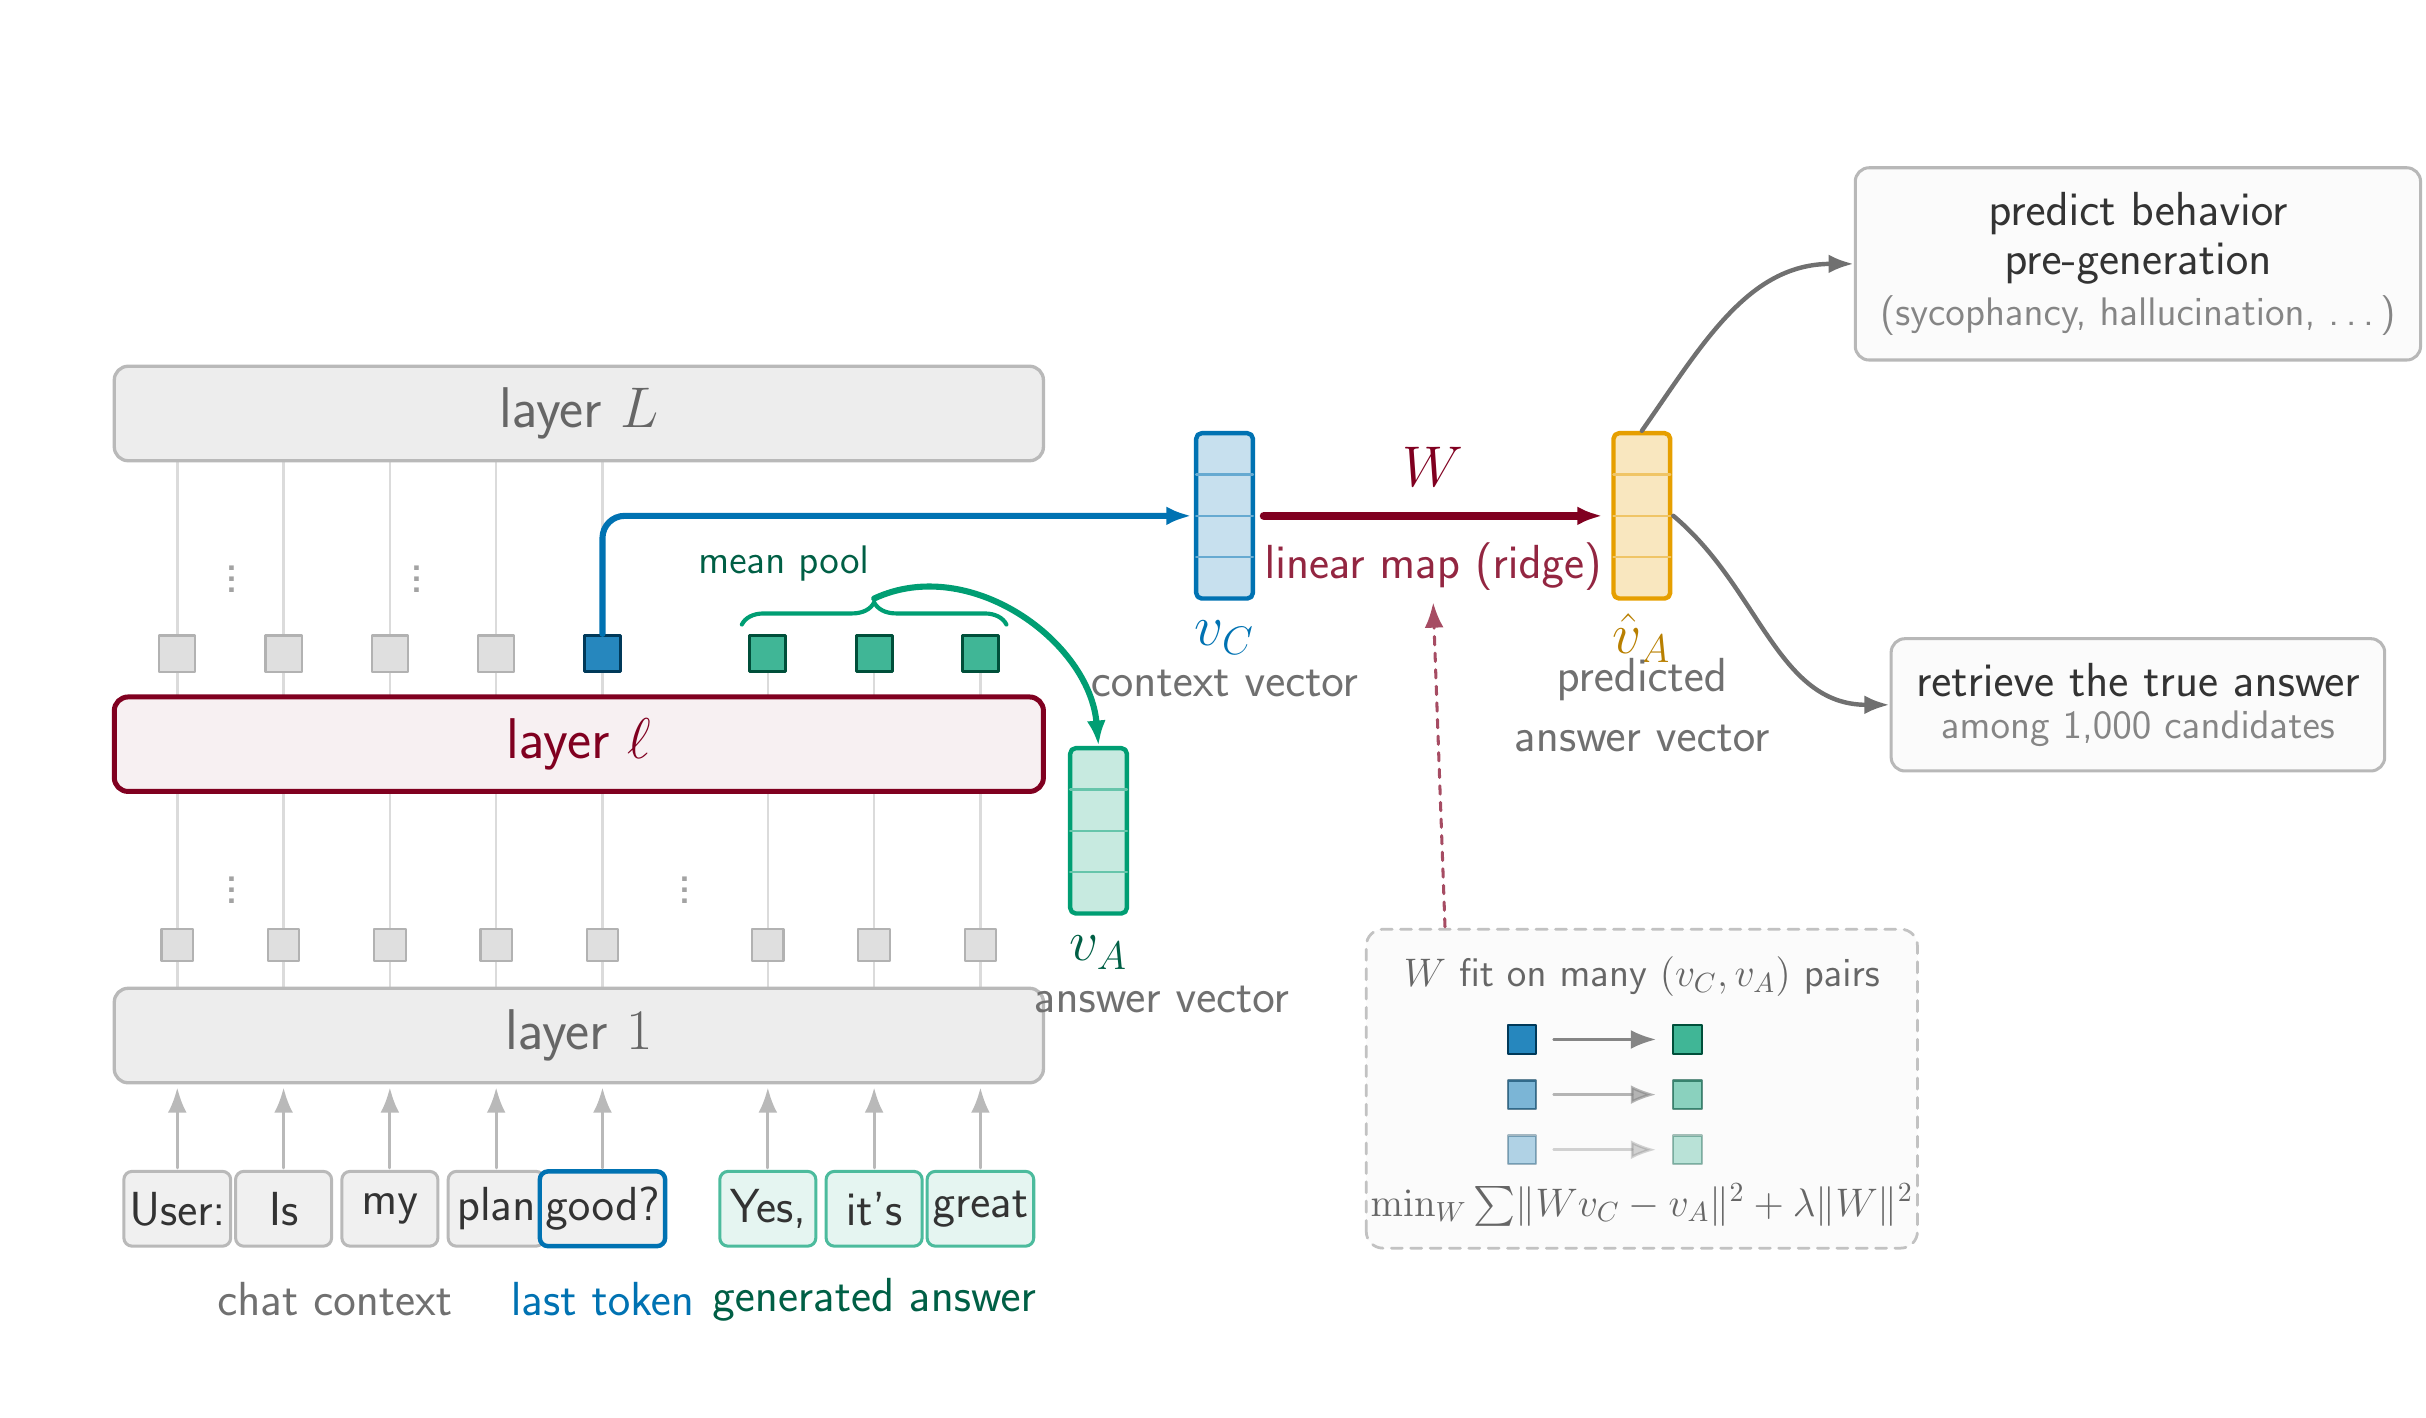
\begin{tikzpicture}[
  >={Latex[length=3.2mm,width=2.4mm]},
  line cap=round, line join=round,
  tok/.style={draw=gray!55, fill=gray!12, rounded corners=3pt, line width=1.1pt,
              minimum height=0.95cm, minimum width=1.22cm, inner sep=2pt,
              font=\LARGE, text=ink},
  layer/.style={draw=gray!55, fill=gray!14, rounded corners=5pt, line width=1.2pt},
  cellg/.style={draw=gray!60, fill=gray!25, line width=0.8pt},
  readout/.style={draw=ink!35, fill=gray!3, rounded corners=5pt, line width=1.1pt,
                  align=center, inner sep=9pt},
]

% ---- canvas (aspect ~1.73) ------------------------------------------------
\useasboundingbox (-0.4,-0.1) rectangle (29.7,17.2);

% ---- residual-stream vertical lines (behind everything) -------------------
\foreach \x in {1.5,2.85,4.2,5.55,6.9,9.0,10.35,11.7}
  \draw[gray!28, line width=0.9pt] (\x,5.0) -- (\x,7.5);
% context columns continue up to layer L; answer columns stop at their tap cells
\foreach \x in {1.5,2.85,4.2,5.55,6.9}
  \draw[gray!28, line width=0.9pt] (\x,8.7) -- (\x,11.7);
\foreach \x in {9.0,10.35,11.7}
  \draw[gray!28, line width=0.9pt] (\x,8.7) -- (\x,9.05);

% ---- transformer layer stack ----------------------------------------------
\draw[layer] (0.7,3.8) rectangle (12.5,5.0);
\node[font=\huge, text=ink!75] at (6.6,4.4) {layer $1$};

\draw[layer, draw=brand, fill=brand!6, line width=1.8pt] (0.7,7.5) rectangle (12.5,8.7);
\node[font=\huge, text=brand] at (6.6,8.1) {layer $\ell$};

\draw[layer] (0.7,11.7) rectangle (12.5,12.9);
\node[font=\huge, text=ink!75] at (6.6,12.3) {layer $L$};

% dots for omitted layers
\node[font=\huge, text=ink!45] at (2.2,6.35) {$\vdots$};
\node[font=\huge, text=ink!45] at (7.95,6.35) {$\vdots$};
\node[font=\huge, text=ink!45] at (2.2,10.3) {$\vdots$};
\node[font=\huge, text=ink!45] at (4.55,10.3) {$\vdots$};

% ---- residual-stream cell rows ---------------------------------------------
% row above layer 1 (all gray)
\foreach \x in {1.5,2.85,4.2,5.55,6.9,9.0,10.35,11.7}
  \draw[cellg] (\x-0.2,5.35) rectangle (\x+0.2,5.75);

% tap row above layer ell
\foreach \x in {1.5,2.85,4.2,5.55}
  \draw[cellg] (\x-0.23,9.02) rectangle (\x+0.23,9.48);
\draw[draw=ctxblue!50!black, fill=ctxblue!85, line width=1.1pt] (6.9-0.23,9.02) rectangle (6.9+0.23,9.48);
\foreach \x in {9.0,10.35,11.7}
  \draw[draw=ansgreen!50!black, fill=ansgreen!75, line width=1.1pt] (\x-0.23,9.02) rectangle (\x+0.23,9.48);

% ---- tokens -----------------------------------------------------------------
\node[tok] at (1.5,2.2) {User:};
\node[tok] at (2.85,2.2) {Is};
\node[tok] at (4.2,2.2) {my};
\node[tok] at (5.55,2.2) {plan};
\node[tok, draw=ctxblue, line width=1.6pt] at (6.9,2.2) {good?};
\node[tok, draw=ansgreen!70, fill=ansgreen!10] at (9.0,2.2) {Yes,};
\node[tok, draw=ansgreen!70, fill=ansgreen!10] at (10.35,2.2) {it's};
\node[tok, draw=ansgreen!70, fill=ansgreen!10] at (11.7,2.2) {great};

% token -> layer 1 arrows
\foreach \x in {1.5,2.85,4.2,5.55,6.9,9.0,10.35,11.7}
  \draw[->, gray!55, line width=1.1pt] (\x,2.72) -- (\x,3.74);

% group labels
\node[font=\LARGE, text=ink!70] at (3.5,1.05) {chat context};
\node[font=\LARGE, text=ctxblue] at (6.9,1.05) {last token};
\node[font=\LARGE, text=ansgreen!60!black] at (10.35,1.05) {generated answer};

% ---- extraction paths --------------------------------------------------------
% v_C: last context token, layer ell
\draw[ctxblue, line width=2.2pt, ->, rounded corners=8pt]
  (6.9,9.5) -- (6.9,11.0) -- (14.38,11.0);

% mean-pool brace over answer cells
\draw[decorate, decoration={brace, amplitude=8pt}, ansgreen, line width=1.5pt]
  (8.67,9.62) -- (12.03,9.62);
\node[font=\Large, text=ansgreen!60!black] at (9.2,10.4) {mean pool};
\draw[ansgreen, line width=2.2pt, ->]
  (10.35,9.95) to[out=25, in=95] (13.2,8.08);

% ---- vector glyphs ------------------------------------------------------------
% v_C
\draw[ctxblue, line width=1.6pt, fill=ctxblue!22, rounded corners=2pt]
  (14.44,9.95) rectangle (15.16,12.05);
\foreach \dy in {10.475,11.0,11.525}
  \draw[ctxblue!60, line width=0.9pt] (14.44,\dy) -- (15.16,\dy);
\node[font=\huge, text=ctxblue] at (14.8,9.45) {$v_C$};
\node[font=\LARGE, text=ink!70] at (14.8,8.88) {context vector};

% v_A
\draw[ansgreen, line width=1.6pt, fill=ansgreen!22, rounded corners=2pt]
  (12.84,5.95) rectangle (13.56,8.05);
\foreach \dy in {6.475,7.0,7.525}
  \draw[ansgreen!60, line width=0.9pt] (12.84,\dy) -- (13.56,\dy);
\node[font=\huge, text=ansgreen!60!black] at (13.2,5.45) {$v_A$};
\node[font=\LARGE, text=ink!70] at (14.0,4.86) {answer vector};

% \hat v_A
\draw[predorange, line width=1.6pt, fill=predorange!25, rounded corners=2pt]
  (19.74,9.95) rectangle (20.46,12.05);
\foreach \dy in {10.475,11.0,11.525}
  \draw[predorange!60, line width=0.9pt] (19.74,\dy) -- (20.46,\dy);
\node[font=\huge, text=predorange!80!black] at (20.1,9.45) {$\hat v_A$};
\node[font=\LARGE, text=ink!70, align=center] at (20.1,8.6) {predicted\\answer vector};

% ---- the map -------------------------------------------------------------------
\draw[brand, line width=3pt, ->] (15.3,11.0) -- (19.6,11.0);
\node[font=\huge, text=brand] at (17.45,11.62) {$W$};
\node[font=\LARGE, text=brand!85] at (17.45,10.35) {linear map (ridge)};

% ---- training inset --------------------------------------------------------------
\draw[draw=ink!30, dash pattern=on 4pt off 3pt, fill=gray!3, rounded corners=6pt, line width=1pt]
  (16.6,1.7) rectangle (23.6,5.75);
\node[font=\Large, text=ink!75] at (20.1,5.15) {$W$ fit on many $(v_C, v_A)$ pairs};
\foreach \yy/\op in {4.35/1.0, 3.65/0.6, 2.95/0.35}{
  \begin{scope}[opacity=\op]
    \draw[draw=ctxblue!50!black, fill=ctxblue!85, line width=0.8pt] (18.4,\yy-0.18) rectangle (18.76,\yy+0.18);
    \draw[->, ink!60, line width=1pt] (18.98,\yy) -- (20.28,\yy);
    \draw[draw=ansgreen!50!black, fill=ansgreen!75, line width=0.8pt] (20.5,\yy-0.18) rectangle (20.86,\yy+0.18);
  \end{scope}
}
\node[font=\Large, text=ink!75] at (20.1,2.25)
  {$\min_W \textstyle\sum \lVert W v_C - v_A \rVert^2 + \lambda \lVert W \rVert^2$};
% connector inset -> W
\draw[brand!70, dash pattern=on 3pt off 3pt, line width=1.1pt, ->]
  (17.6,5.78) -- (17.45,9.9);

% ---- readouts ---------------------------------------------------------------------
\node[readout] (rA) at (26.4,14.2)
  {\LARGE\textcolor{ink}{predict behavior}\\[2pt]
   \LARGE\textcolor{ink}{pre-generation}\\[3pt]
   \Large\textcolor{ink!60}{(sycophancy, hallucination, \dots)}};
\node[readout] (rB) at (26.4,8.6)
  {\LARGE\textcolor{ink}{retrieve the true answer}\\[3pt]
   \Large\textcolor{ink!60}{among 1{,}000 candidates}};

\draw[ink!70, line width=1.6pt, ->] (20.1,12.08) to[out=55, in=180] (rA.west);
\draw[ink!70, line width=1.6pt, ->] (20.5,11.0) to[out=-40, in=180] (rB.west);

\end{tikzpicture}
\end{document}
